\documentclass[paper=a4, fontsize=10pt]{scrartcl} % A4 paper and 11pt font size

\usepackage[T1]{fontenc} % Use 8-bit encoding that has 256 glyphs
\usepackage{fourier} % Use the Adobe Utopia font for the document - comment this line to return to the LaTeX default
\usepackage[english]{babel} % English language/hyphenation
\usepackage{amsmath,amsfonts,amsthm} % Math packages
\usepackage{graphicx}
\usepackage[cm]{fullpage}
\usepackage{float}
\usepackage{sectsty} % Allows customizing section commands
\usepackage{subcaption}

\usepackage{minted}

\renewcommand{\theFancyVerbLine}{
  \sffamily\textcolor[rgb]{0.5,0.5,0.5}{\scriptsize\arabic{FancyVerbLine}}}

\allsectionsfont{\centering \normalfont\scshape} % Make all sections centered, the default font and small caps

\usepackage{fancyhdr} % Custom headers and footers
\pagestyle{fancyplain} % Makes all pages in the document conform to the custom headers and footers
\fancyhead{} % No page header - if you want one, create it in the same way as the footers below
\fancyfoot[L]{} % Empty left footer
\fancyfoot[C]{} % Empty center footer
\fancyfoot[R]{\thepage} % Page numbering for right footer
\renewcommand{\headrulewidth}{0pt} % Remove header underlines
\renewcommand{\footrulewidth}{0pt} % Remove footer underlines
\setlength{\headheight}{13.6pt} % Customize the height of the header

\numberwithin{equation}{section} % Number equations within sections (i.e. 1.1, 1.2, 2.1, 2.2 instead of 1, 2, 3, 4)
\numberwithin{figure}{section} % Number figures within sections (i.e. 1.1, 1.2, 2.1, 2.2 instead of 1, 2, 3, 4)
\numberwithin{table}{section} % Number tables within sections (i.e. 1.1, 1.2, 2.1, 2.2 instead of 1, 2, 3, 4)

\setlength\parindent{0pt} % Removes all indentation from paragraphs - comment this line for an assignment with lots of text

%----------------------------------------------------------------------------------------
%	TITLE SECTION
%----------------------------------------------------------------------------------------

\newcommand{\horrule}[1]{\rule{\linewidth}{#1}} % Create horizontal rule command with 1 argument of height

\newtoks\rowvectoks
\newcommand{\rowvec}[2]{%
  \rowvectoks={#2}\count255=#1\relax
  \advance\count255 by -1
  \rowvecnexta}
\newcommand{\rowvecnexta}{%
  \ifnum\count255>0
    \expandafter\rowvecnextb
  \else
    \begin{pmatrix}\the\rowvectoks\end{pmatrix}
  \fi}
\newcommand\rowvecnextb[1]{%
    \rowvectoks=\expandafter{\the\rowvectoks&#1}%
    \advance\count255 by -1
    \rowvecnexta}

\title{	
\normalfont \normalsize 
\textsc{Radboud University Nijmegen}  % Your university, school and/or department name(s)
\horrule{0.5pt} \\[0.3cm] % Thin top horizontal rule
\huge Statistical Machine Learning \\ Assignment 4 \\ % The assignment title
\horrule{2pt}  % Thick bottom horizontal rule
}

\author{Steven Reitsma \\ (s4132343)} % Your name

\date{\normalsize\today} % Today's date or a custom date

\begin{document}

\maketitle % Print the title

\section{EM and doping}
\subsection{Visualizing the data}
Plotting $x_1$ on the x-axis, $x_2$ on the y-axis, and the sum of $x_3$ and $x_4$ as the color gives the plot as shown in Figure \ref{visualization}. We can definitely see some structure in the data, annotated in Figure \ref{visualization_annotated}. If we plot the variables in 3d-space, with $x_1$ on the x-axis, $x_2$ on the y-axis, $x_3$ on the z-axis and $x_4$ as color, we can see that there is a cloud of points that forms a perpendicular plane to the other cloud of points. This is the same cloud of points that is visible in the 2d-plot as the purple class (see Figure \ref{visualization_annotated}). The 3d-visualization can be shown by running the \verb|exercise_11_3d.py| file (requires \verb|matplotlib| and \verb|mpltools|).

\begin{figure}[h!]
	\centering
	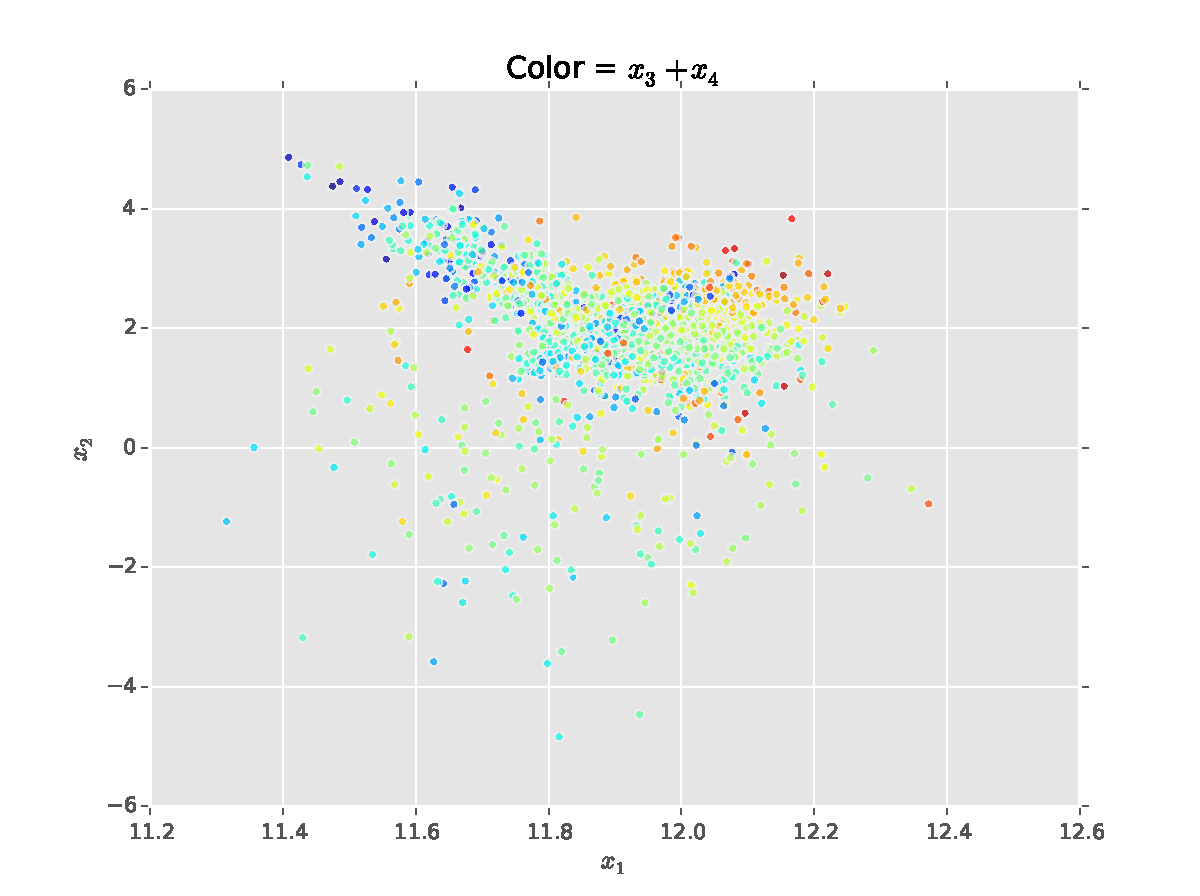
\includegraphics[width=0.75\textwidth]{exercise_11.pdf}
	\caption{Plot of the data set with $x_1$ on the x-axis, $x_2$ on the y-axis, and $x_3 + x_4$ as the color.}
	\label{visualization}
\end{figure}

\begin{figure}[h!]
	\centering
	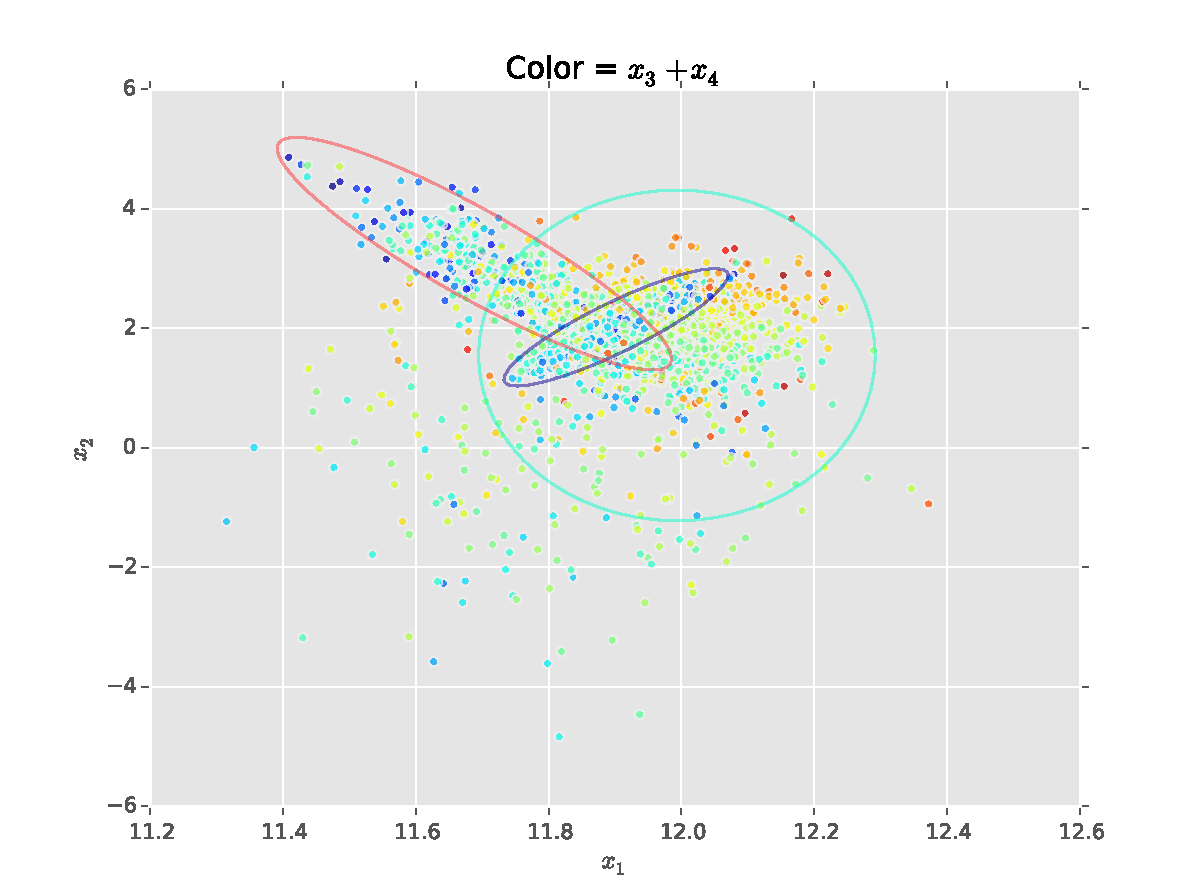
\includegraphics[width=\textwidth]{exercise_11_annotated.pdf}
	\caption{The different classes that can be observed in the data. The cyan class is the largest one, where there is no correlation between $x_1$ and $x_2$. The purple class has a positive correlation between $x_1$ and $x_2$, while the orange class has a negative correlation between $x_1$ and $x_2$. The purple and cyan classes can be distinguished easily using $x_3$ and $x_4$. Seperating the orange class seems harder.}
	\label{visualization_annotated}
\end{figure}
\subsection{Implementing the algorithm}
Instead of coding the equations in Bishop 9.2.2 directly I vectorized some of them so the algorithm would run faster and the operations are (in my opinion) easier to understand. I have included the EM algorithm code below. It is fairly straight forward and heavily commented.

\begin{minted}[mathescape,
               linenos,
               numbersep=5pt,
               gobble=0,
               frame=lines,
               framesep=2mm,
               fontsize=\footnotesize]{python}
import numpy as np
import matplotlib.pyplot as plt
from mpltools import style
from scipy.stats import multivariate_normal
style.use('ggplot')

def gaussian(x, mu, sigma):
	"""
	This is the pdf for the Gaussian defined by mu and sigma for a certain sample x.
	"""
	normalizer = 1. / (2*np.pi)**(x.shape[0]/2) * 1. / np.sqrt(np.linalg.det(sigma))
	return normalizer * np.exp(-1./2 * np.dot(x - mu, np.dot(np.linalg.inv(sigma), x - mu)))
	# Scipy method below: significantly slower than implementation above, results are equal
	# return multivariate_normal.pdf(x, mu, sigma)

def loglikelihood(pi, mu, sigma, data):
	"""
	Computes the log likelihood as a function of the mixing coefficients, mu, sigma and the data.
	"""
	return np.sum([np.log(np.sum([pi[k] * gaussian(x, mu[k], sigma[k]) for k in range(0, K)])) for x in data])

def EM(data, K, iterations = 100, min_delta = 1.0e-4):
	"""
	Runs the EM algorithm on data with K classes for a set amount of iterations (default is 100).
	The min_delta parameter sets the minimum log likelihood difference per iteration.
	If the difference between two iterations is smaller than this value, the algorithm is stopped early.
	"""
	# Initialize mu to the mean of the data set +- a random value between 0 and 1
	mu = [np.ravel(np.mean(data, 0) + np.random.rand(1, data.shape[1]) * 2 - 1) for _ in range(0, K)]

	# Initialize sigma to a diagonal matrix with random numbers between 2 and 6 on the diagonals.
	sigma = [np.diagflat(np.random.rand(1, data.shape[1]) * 4 + 2) for _ in range(0, K)]

	# Initialize equal mixing coefficients
	pi = np.repeat(1. / K, K)

	# Initialize gamma array
	gamma = np.zeros((data.shape[0], K))
	previous_loglikelihood = 0

	for i in range(0, iterations):
		# Check for convergence
		current_loglikelihood = loglikelihood(pi, mu, sigma, data)
		if np.abs(previous_loglikelihood - current_loglikelihood) < min_delta:
			# We have converged well enough
			print "Stopping early because of convergence after %i iterations." % i
			break

		# Recompute log likelihood and print it
		previous_loglikelihood = current_loglikelihood
		print "Log likelihood: %.2f" % current_loglikelihood

		# Compute unnormalized gamma values for each class for each data point.
		# We normalize later, because part of the normalization coefficient has
		# to be calculated later on anyway (for the other class).
		# Doing it now would mean we have to calculate it multiple times.
		for k in range(0, K):
			gamma[:, k] = [pi[k] * gaussian(sample, mu[k], sigma[k]) for sample in data]

		# Normalize the gamma values
		gamma = gamma / np.repeat(np.sum(gamma, 1)[np.newaxis], K, axis=0).T

		# Compute N
		N = np.sum(gamma, 0)

		# M step, compute mu and sigma for each class/Gaussian
		for k in range(0, K):
			mu[k] = 1./N[k] * np.dot(gamma[:, k], data)
			sigma[k] = 1./N[k] * np.dot(gamma[:, k], (data - mu[k])[np.newaxis].T * (data - mu[k])[np.newaxis])

		# Recompute the mixing coefficients
		pi = N / np.sum(N)

	# Print the final log likelihood, the final distribution and show the plot
	print "Final log likelihood: %.2f" % loglikelihood(pi, mu, sigma, data)
	print "Final distribution (red, blue, purple, green, pink, gray, yellow): %s" % pi
	plot(data, gamma)

def plot(data, gamma):
	# First make some normal colors
	color_cycle = ['#E24A33', '#348ABD', '#988ED5', '#8EBA42', '#FFB5B8', '#777777', '#FBC15E']

	assert gamma.shape[1] <= len(color_cycle)

	plt.scatter(data[:, 0], data[:, 1], c = [color_cycle[x] for x in np.argmax(gamma, 1)], alpha = 0.75)
	plt.show()

if __name__ == "__main__":
	data = np.loadtxt('data/a011_mixdata.txt')
	K = 4

	EM(data, K)
\end{minted}

\subsection{Two classes}
For $K = 2$, the log likelihood converges to $-7058.13$. The data points plotted in 2d space (with $x_1$ and $x_2$), colored according to the most likely class are shown in Figure \ref{k2}. $33.0\%$ of the data points are in the red class and $67.0\%$ in the blue class. I have tried multiple runs and get rougly the same result each time (although the colors switch around of course). Using the code snippet below I get a correlation of $-0.053$ for the blue class and a correlation of $-0.32$ for the red class. This means there is no correlation in the blue class, and a medium negative correlation in the red class. Neither class shows the characteristic strong positive correlation between $x_1$ and $x_2$. Therefore it is safe to say that the data is not made up of only two Gaussians.

\begin{minted}[mathescape,
               linenos,
               numbersep=5pt,
               gobble=0,
               frame=lines,
               framesep=2mm,
               fontsize=\footnotesize]{python}
	correlation = [sigma[k][0, 1] / np.sqrt(sigma[k][0, 0] * sigma[k][1, 1]) for k in range(0, K)]
\end{minted}

\begin{figure}[h!]
	\centering
	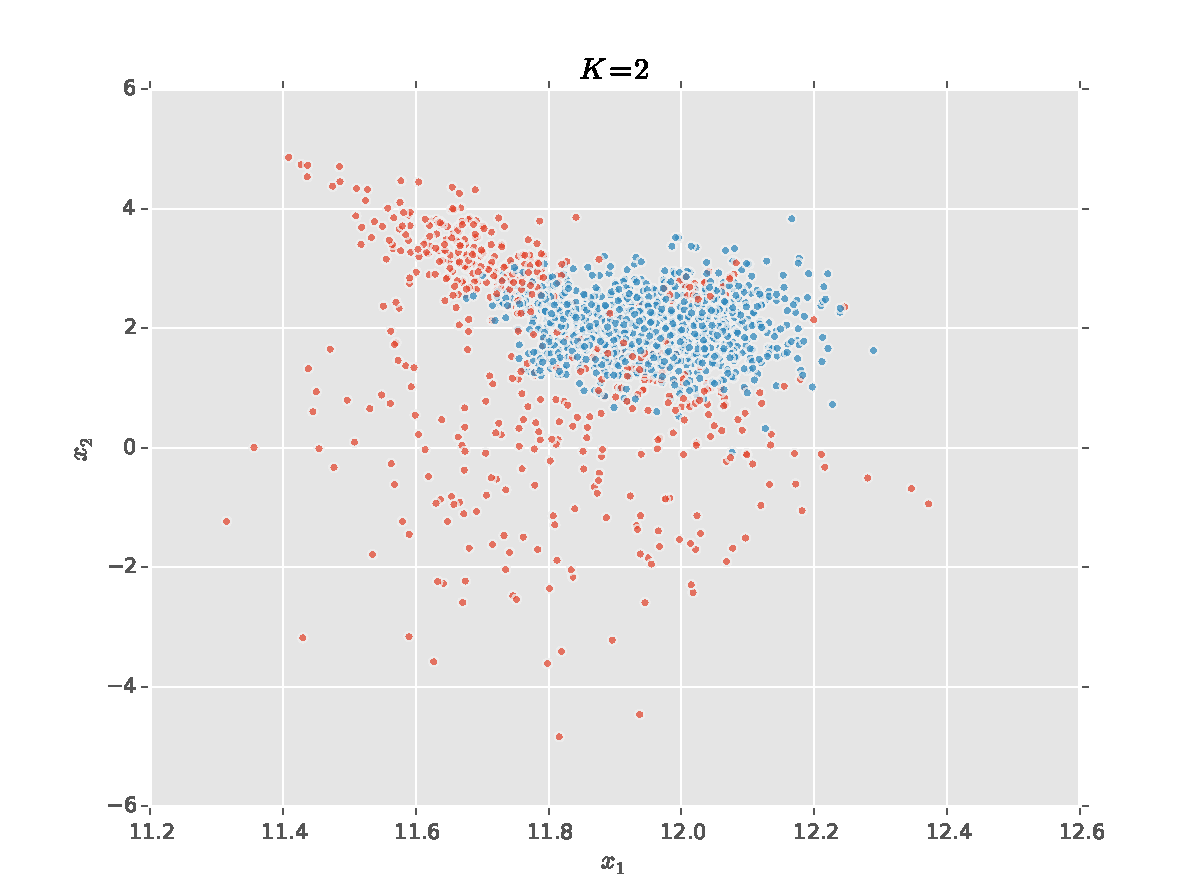
\includegraphics[width=\textwidth]{exercise_13.pdf}.
	\caption{The data points colored after their most likely cluster assignment for $K = 2$.}
	\label{k2}
\end{figure}

\subsection{More classes}
For $K=3$ the log likelihood converges to a value of $-6551.13$. The plot is shown in Figure \ref{k3}. The correlations for the red, blue and purple classes are respectively: 0.081, -0.72 and -0.017. Still, there is no strong positive correlation in the components.

\begin{figure}[H]
	\centering
	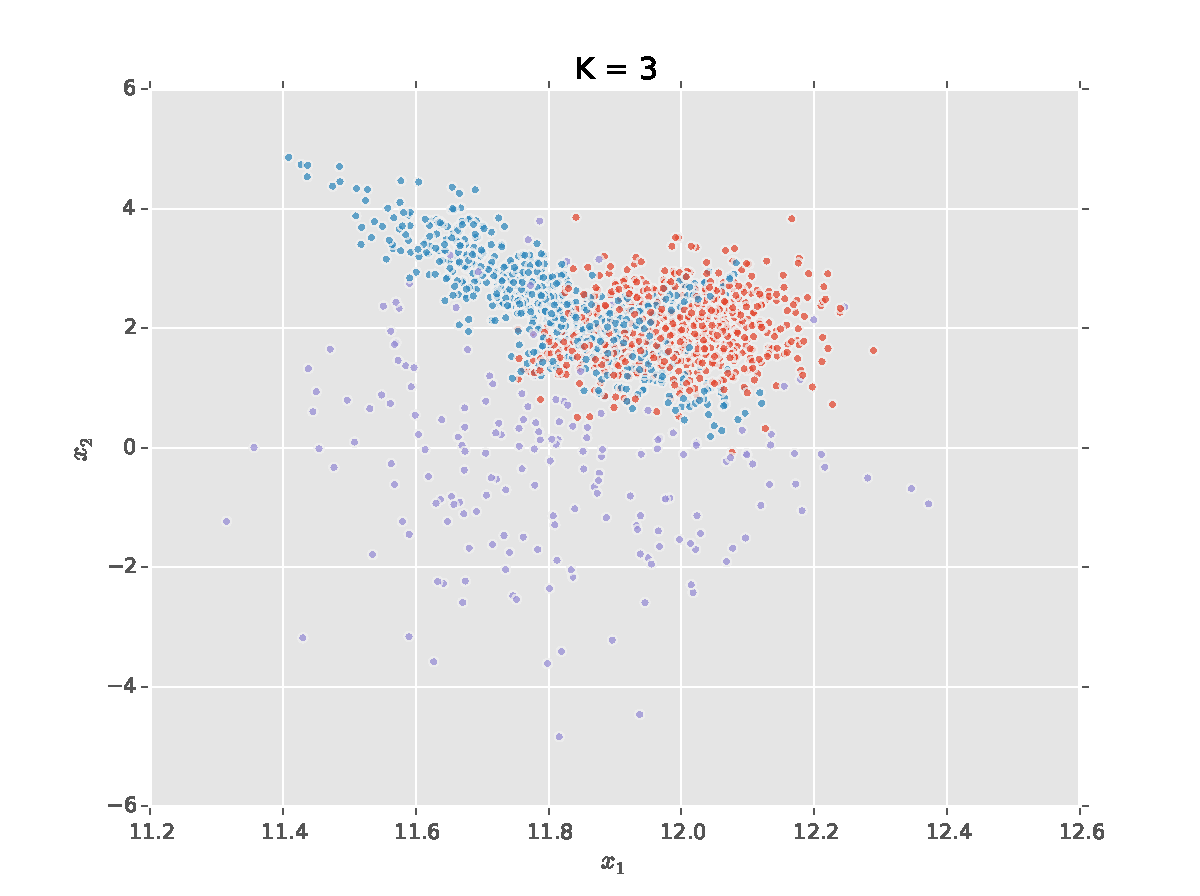
\includegraphics[width=0.7\textwidth]{exercise_14a.pdf}
	\caption{The data points colored after their most likely cluster assignment for $K = 3$.}
	\label{k3}
\end{figure}

For $K = 4$ we get our most interesting results. The log likelihood converges to $-5989.75$. The plot is shown in Figure \ref{k4}. The correlations for the red, blue, purple and green classes are respectively: 0.92, -0.053, 0.036, -0.89. These show the strong positive correlation between $x_1$ and $x_2$ in the red class and the strong negative correlation that was hypothesized as a possible group for clean athletes in the green class. It seems that my initial guess of the data containing only three classes was incorrect. From the plots for various values of $K$ we can assume that $K=4$ is the most likely case. The portion of all data points in the red class (i.e. the final value of $\pi_{red}$) is $0.196$. Therefore it is safe to say that the estimate of 20\% of the users using doping is quite correct.

\begin{figure}[H]
	\centering
	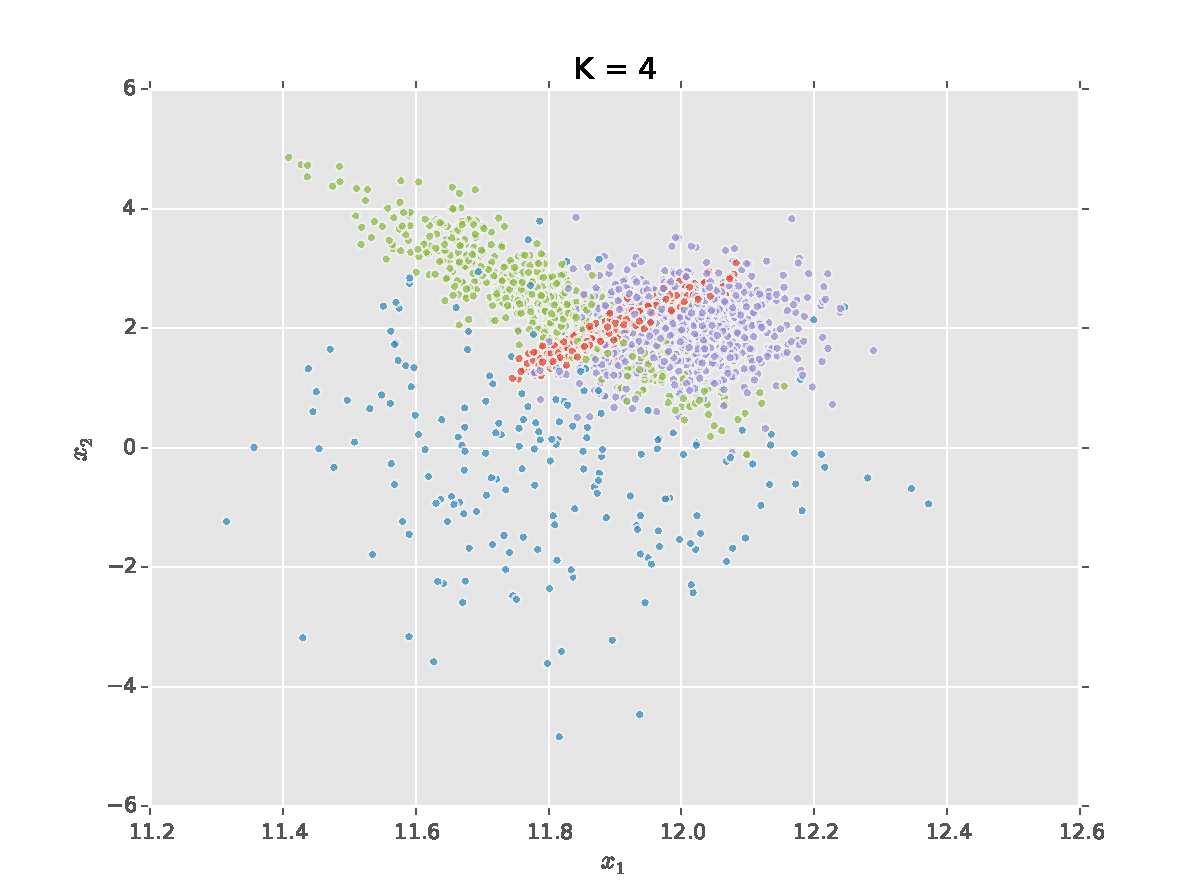
\includegraphics[width=0.7\textwidth]{exercise_14b.pdf}
	\caption{The data points colored after their most likely cluster assignment for $K = 4$.}
	\label{k4}
\end{figure}

\subsection{Samples}
Using the code snippet below, we get the following result:

\begin{minted}[mathescape,
               linenos,
               numbersep=5pt,
               gobble=0,
               frame=lines,
               framesep=2mm,
               fontsize=\footnotesize]{python}
A = np.array([11.85, 2.2, 0.5, 4.0])
A_likelihood = [pi[k] * gaussian(A, mu[k], sigma[k]) for k in range(0, K)]
A_likelihood /= np.sum(A_likelihood)
print "Likelihoods for sample A: %s" % A_likelihood
\end{minted}

\begin{itemize}
\item A belongs to the purple class (in Figure \ref{k4}) with a confidence of 0.583.
\item B belongs to the green class with a confidence of 0.920.
\item C belongs to the red class with a confidence of 0.999.
\item D belongs to the purple class with a confidence of 0.993.
\end{itemize}

Therefore, it is safe to say that C is from a subject who took drug X, since this data point belongs to the class with the strong positive correlation. Furthermore I would say that A is from a subject who tried to tamper with the test, since the confidence is lower. Sample B has a high confidence for the (green) class with a strong negative correlation. This class is hypothesized to include clean athletes as mentioned in the introduction of the assignment. So B is clean. Sample D has a very high confidence for the purple (non correlated) class, so D is clean too.

\section{Handwritten digit recognition}
\subsection{Showing images}
I used the following piece of code to read and show images:
\begin{minted}[mathescape,
               linenos,
               numbersep=5pt,
               gobble=0,
               frame=lines,
               framesep=2mm,
               fontsize=\footnotesize]{python}
def readData():
	"""
	Reads the input binary file.
	"""
	N = 800
	D = 28*28
	X = np.zeros((N, D), dtype=np.uint8)

	f = open("data/a012_images.dat", 'rb')

	for i in range(0, N):
		X[i, :] = np.fromstring(f.read(D), dtype='uint8')

	f.close()

	return X

if __name__ == "__main__":
	X = readData()
	
	img = plt.imshow(X[0, :].reshape(28, 28, order='F')) # Fortran order is required for MATLAB compliance
	img.set_interpolation('nearest')
	img.set_cmap('gray')
	plt.show()
\end{minted}

In Figure \ref{digits} I have put some examples of the digits.

\begin{figure}[H]
	\centering
	\begin{subfigure}[b]{0.3\textwidth}
                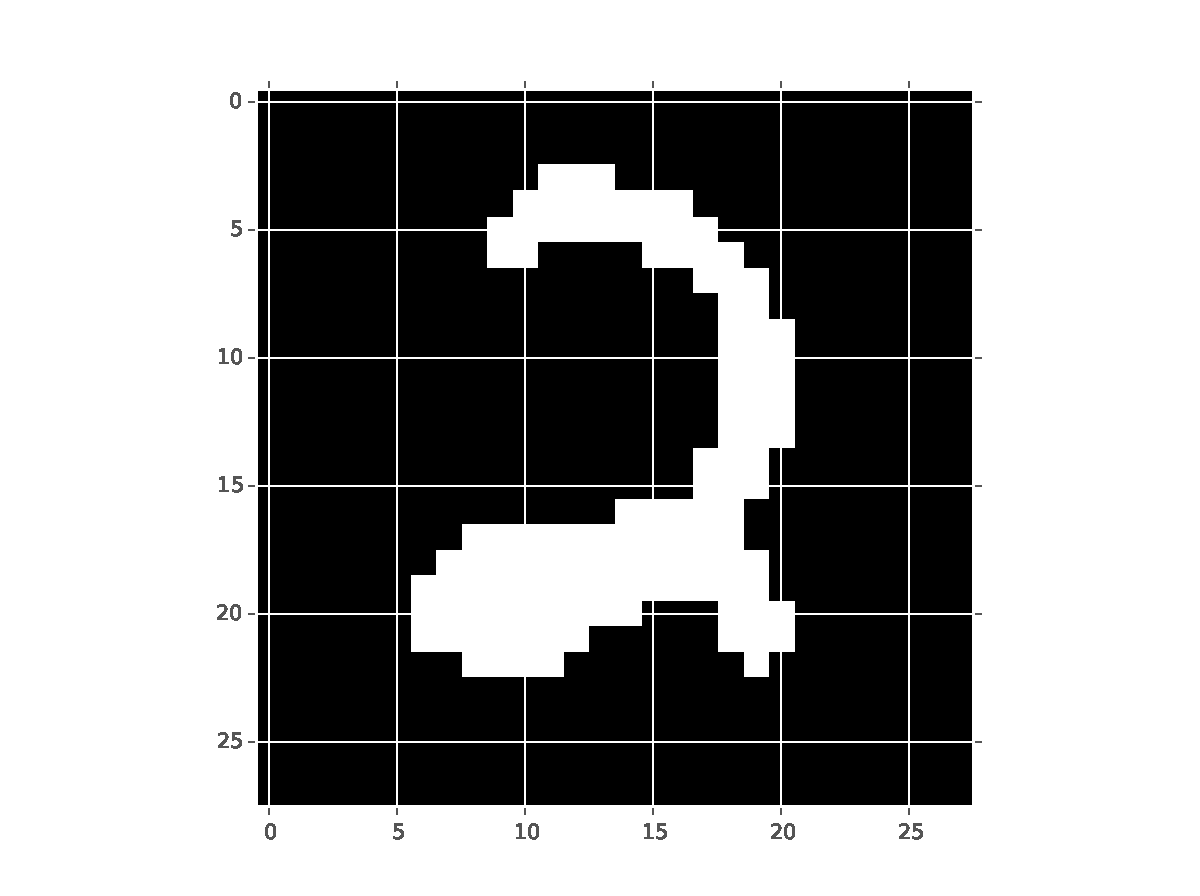
\includegraphics[width=\textwidth]{two}
                \caption{A two.}
        \end{subfigure}%
        ~ %add desired spacing between images, e. g. ~, \quad, \qquad, \hfill etc.
          %(or a blank line to force the subfigure onto a new line)
        \begin{subfigure}[b]{0.3\textwidth}
                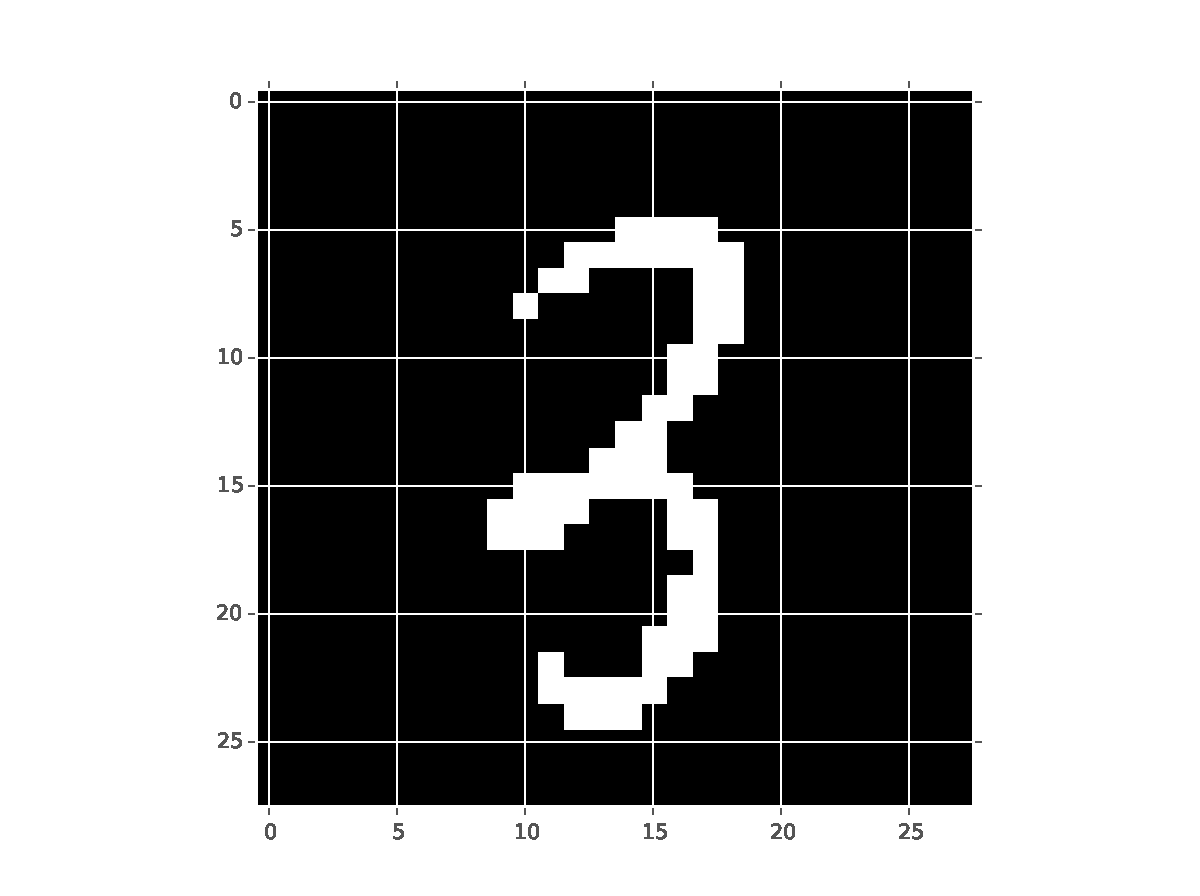
\includegraphics[width=\textwidth]{three}
                \caption{A three.}
        \end{subfigure}
        ~ %add desired spacing between images, e. g. ~, \quad, \qquad, \hfill etc.
          %(or a blank line to force the subfigure onto a new line)
        \begin{subfigure}[b]{0.3\textwidth}
                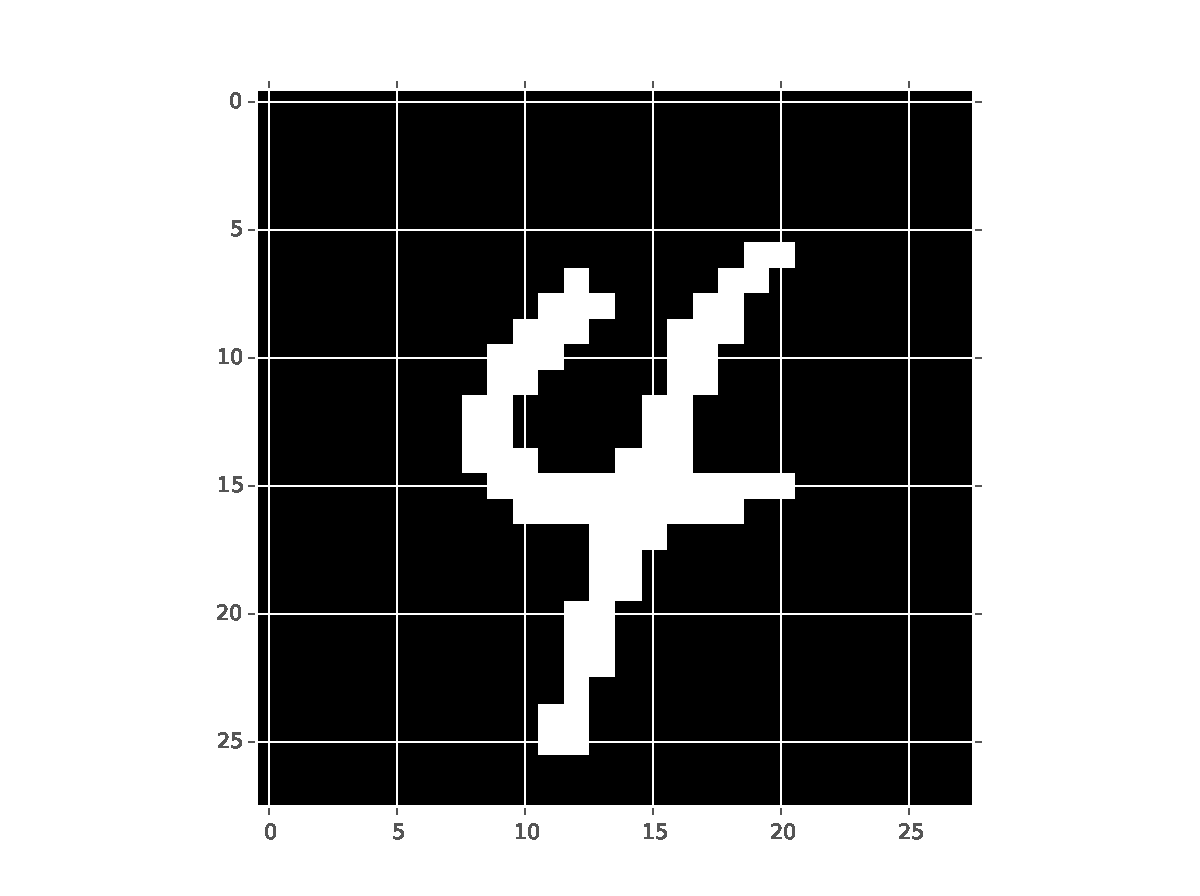
\includegraphics[width=\textwidth]{four}
                \caption{A four.}
        \end{subfigure}
        \caption{Some examples of the digits in the data set.}
        \label{digits}
\end{figure}

I think it will be possible to classify the digits correctly with a class prototype to a certain extent. There is however a lot of variance in the digits so not all digits will be classified correctly.

\subsection{Implementation}
The relevant code can be found below. The algorithm is very similar to the algorithm that was used in the first exercise. The only difference being that a Bernoulli pdf is used instead of a Gaussian, and the computation of $\Sigma$ is omitted. I had no problems with likelihood values that got too small. Apparently \verb|numpy| floats have a very high precision. Note that the code snippet below does not show code that was reused from the algorithm in exercise 1. The full code can be found in \verb|exercise_22.py| and the code listing.

\begin{minted}[mathescape,
               linenos,
               numbersep=5pt,
               gobble=0,
               frame=lines,
               framesep=2mm,
               fontsize=\footnotesize]{python}
from exercise_21 import readData

def bernoulli(x, mu):
	"""
	This is the pdf for the Bernoulli defined by mu for a certain sample x.
	"""
	return np.product(mu**x * (1-mu)**(1-x))

def loglikelihood(pi, mu, data, K):
	"""
	Computes the log likelihood as a function of the mixing coefficients, mu, sigma and the data.
	"""
	return np.sum(np.log([np.sum([pi[k] * bernoulli(x, mu[k]) for k in range(0, K)]) for x in data]))

def EM(data, K, iterations = 100, min_delta = 1.0e-4):
	"""
	[...]
	"""
	# Initialize equal mixing coefficients
	[...]

	# Initialize gamma array
	[...]

	for i in range(0, iterations):
		# Check for convergence
		[...]
		# Recompute log likelihood and print it
		[...]

		# Compute unnormalized gamma values for each class for each data point.
		# [...]
		for k in range(0, K):
			gamma[:, k] = [pi[k] * bernoulli(sample, mu[k]) for sample in data]

		# Normalize the gamma values
		[...]

		# Compute N
		[...]

		# M step, compute mu for each class/Gaussian
		for k in range(0, K):
			mu[k] = [...]
			# Removed sigma computation

		# Recompute the mixing coefficients
		[...]

if __name__ == "__main__":
	data = readData()
	K = 3

	EM(data, K, iterations = 100)
\end{minted}

As a bonus I tested the performance of calculating $p(\boldsymbol x \vert \boldsymbol \mu_k)$ using equation 9.48 from Bishop and using a vectorized equivalent. The two code snippets are shown below and the table with the performance results is shown in Table \ref{vectorize}. The output of the two methods is the same.

According to equations 9.48, unvectorized:
\begin{minted}[mathescape,
               linenos,
               numbersep=5pt,
               gobble=0,
               frame=lines,
               framesep=2mm,
               fontsize=\footnotesize]{python}
np.product([mu[i]**x[i] * (1-mu[i])**(1-x[i]) for i in range(0, x.shape[0])])
\end{minted}

Vectorized equivalent:
\begin{minted}[mathescape,
               linenos,
               numbersep=5pt,
               gobble=0,
               frame=lines,
               framesep=2mm,
               fontsize=\footnotesize]{python}
np.product(mu**x * (1-mu)**(1-x))
\end{minted}

\begin{table}[h!]
	\centering
	\begin{tabular}{|l|l|}
		\hline
		\textbf{Unvectorized} & 0.166 iterations per second \\
		\textbf{Vectorized} & 5.06 iterations per second \\
		\hline
	\end{tabular}
	\caption{Performance results for the unvectorized and vectorized versions of the same equation. N = 10. Speed up: 30x.}
	\label{vectorize}
\end{table}

\subsection{Running the algorithm}
In Figure \ref{means_digits} the means of the three EM clusters are shown. We can clearly see that the means represent the digits 3, 2 and 4, respectively. After running the algorithm with some different initializations I can conclude that the three different digits are almost always found. An exception is shown in Figure \ref{bad_digits}, where the first cluster prototype is a hybrid between a 2 and a 4.

\begin{figure}[H]
	\centering
	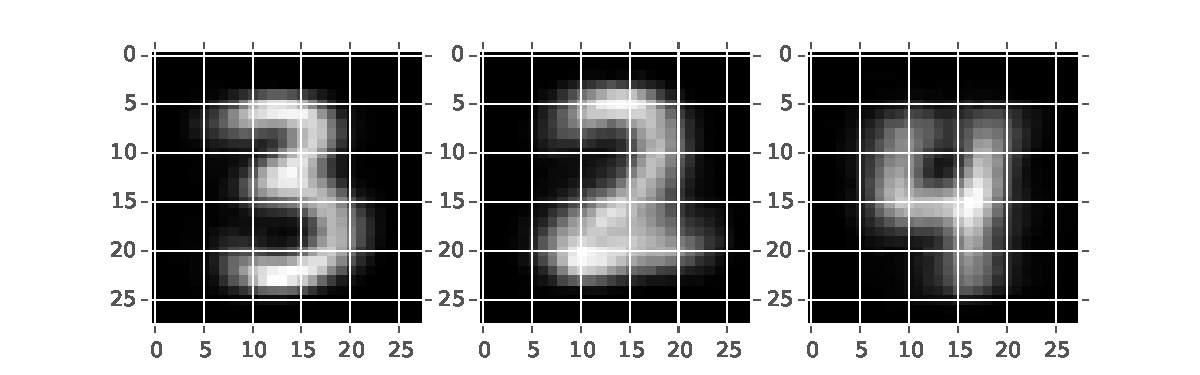
\includegraphics[width=0.7\textwidth]{means_digits.pdf}
	\caption{The means of the EM clusters trained on the digits data set for $K = 3$.}
	\label{means_digits}
\end{figure}

\begin{figure}[H]
	\centering
	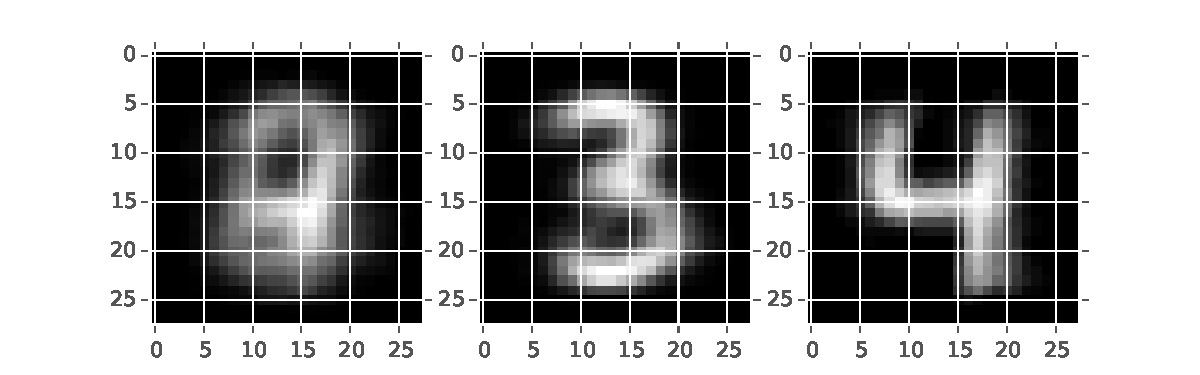
\includegraphics[width=0.7\textwidth]{bad.pdf}
	\caption{An example of bad results achieved using the EM algorithm. Shown are the means of the EM clusters trained on the digits data set for $K = 3$.}
	\label{bad_digits}
\end{figure}

\subsection{Changes to the parameters}
\subsubsection{Different class amounts}

If we use $K > 3$ we get interesting results. Most of the time, we get cluster prototypes for different variations of the same digit, e.g. a curly 2 vs. a straight 2 or a closed 4 vs. an open 4. In some of the cases, the mixing coefficient $\pi$ is driven to zero, which makes the prototype unresponsive to any changes. See Figure \ref{low_pi} for an example. A solution to this would be to reinitialize the mean for a class to a new random value if the mixing coefficient $\pi$ is very low. The same issue is present in the K-means algorithm, and the same solution can be applied and works relatively well\footnote{This is actually the method that scikit-learn uses as well in their MiniBatchKMeans implementation. See \url{https://github.com/scikit-learn/scikit-learn/blob/master/sklearn/cluster/k\_means\_.py} for more information.}.

\begin{figure}[H]
	\centering
	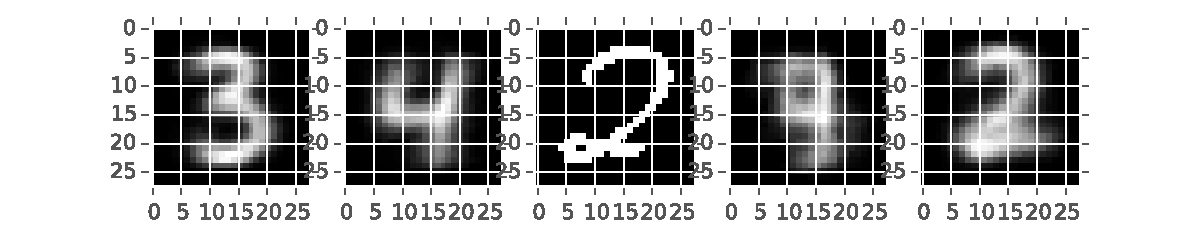
\includegraphics[width=0.7\textwidth]{bad2.pdf}
	\caption{An example of a cluster prototype (third) that has not changed since its first iteration due to a very low mixing coefficient $\pi$. Shown are the means of the EM clusters trained on the digits data set for $K = 5$.}
	\label{low_pi}
\end{figure}

If we use fewer than 3 classes, the phenomenon of hybrids becomes more prevalent. See Figure \ref{hybrid}, where the second cluster prototype is a hybrid between a 2 and a 4.

\begin{figure}[H]
	\centering
	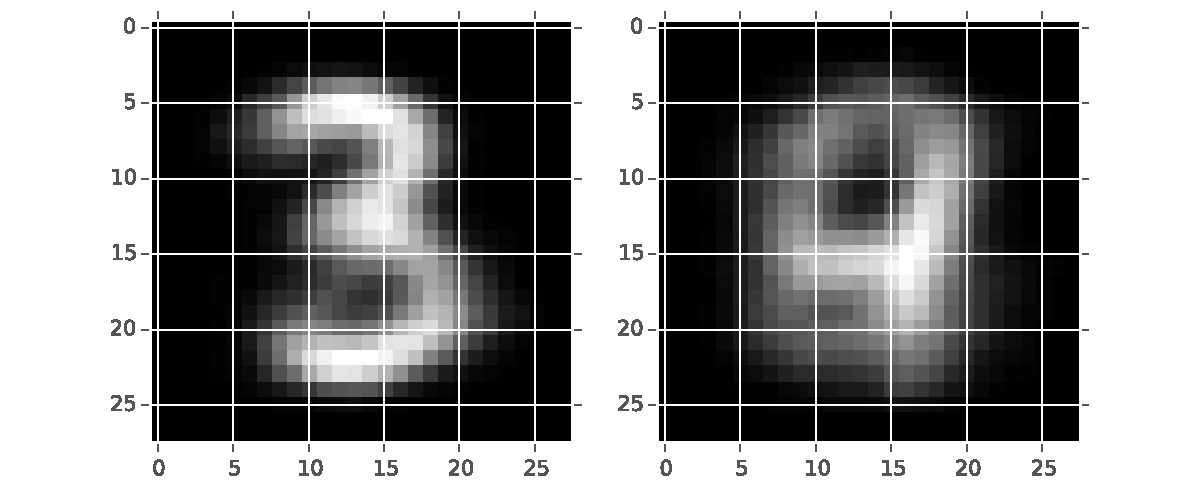
\includegraphics[width=0.7\textwidth]{hybrid_2.pdf}
	\caption{Shown are the means of the EM clusters trained on the digits data set for $K = 2$. Notice the hybrid prototype in the second picture.}
	\label{hybrid}
\end{figure}

\subsubsection{Checking the labels}
Using the labels we can get a classification error. From several tests the classification error seems to be between 8 and 15 percent. This is actually quite high; definitely higher than I anticipated. In Figure \ref{error_digits} some misclassified digits are shown for the prototypes as shown in Figure \ref{error_prototypes}. Some of the errors are in digits that can be very obviously classified by humans, but of course it's not that easy for algorithms (see the second digit below).

\begin{figure}[H]
	\centering
	\begin{subfigure}[b]{0.3\textwidth}
                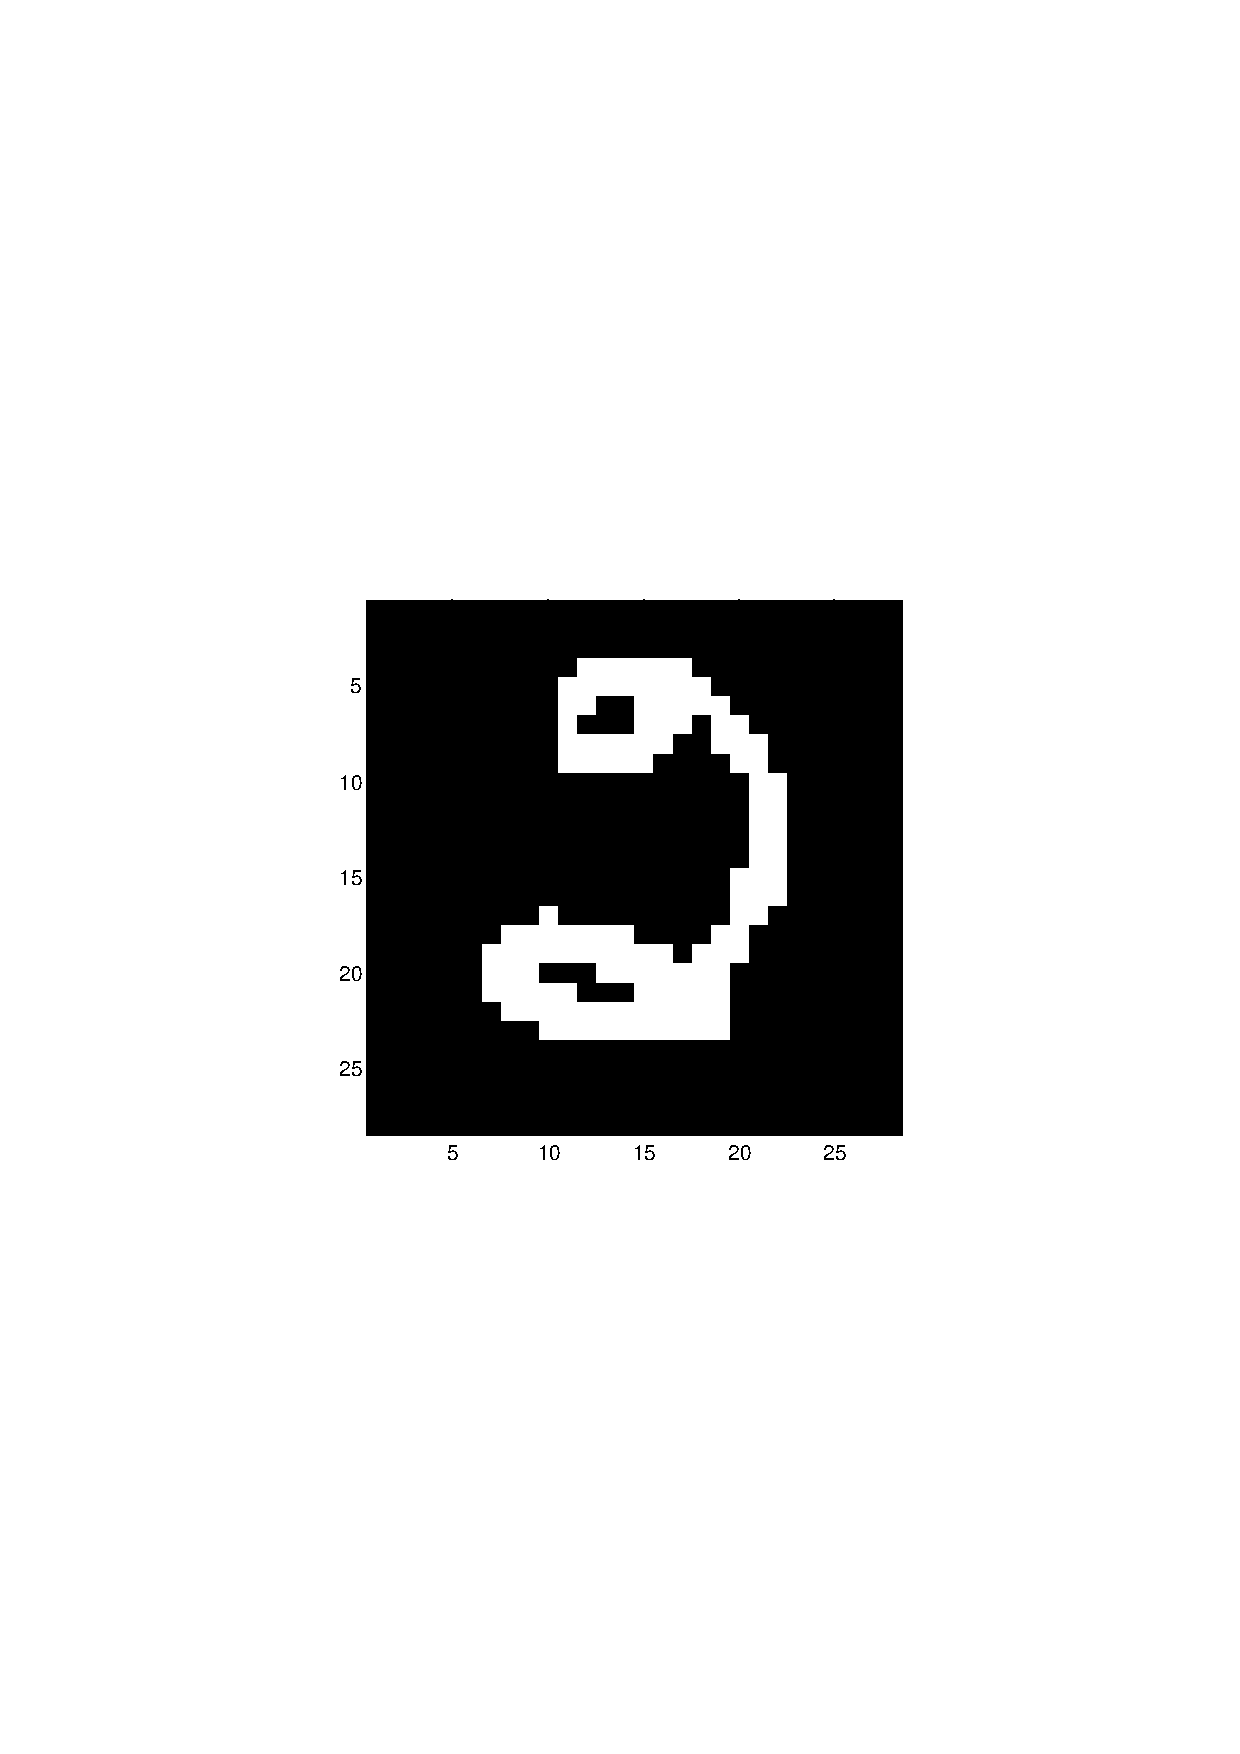
\includegraphics[width=\textwidth]{error_1}
        \end{subfigure}%
        ~ %add desired spacing between images, e. g. ~, \quad, \qquad, \hfill etc.
          %(or a blank line to force the subfigure onto a new line)
        \begin{subfigure}[b]{0.3\textwidth}
                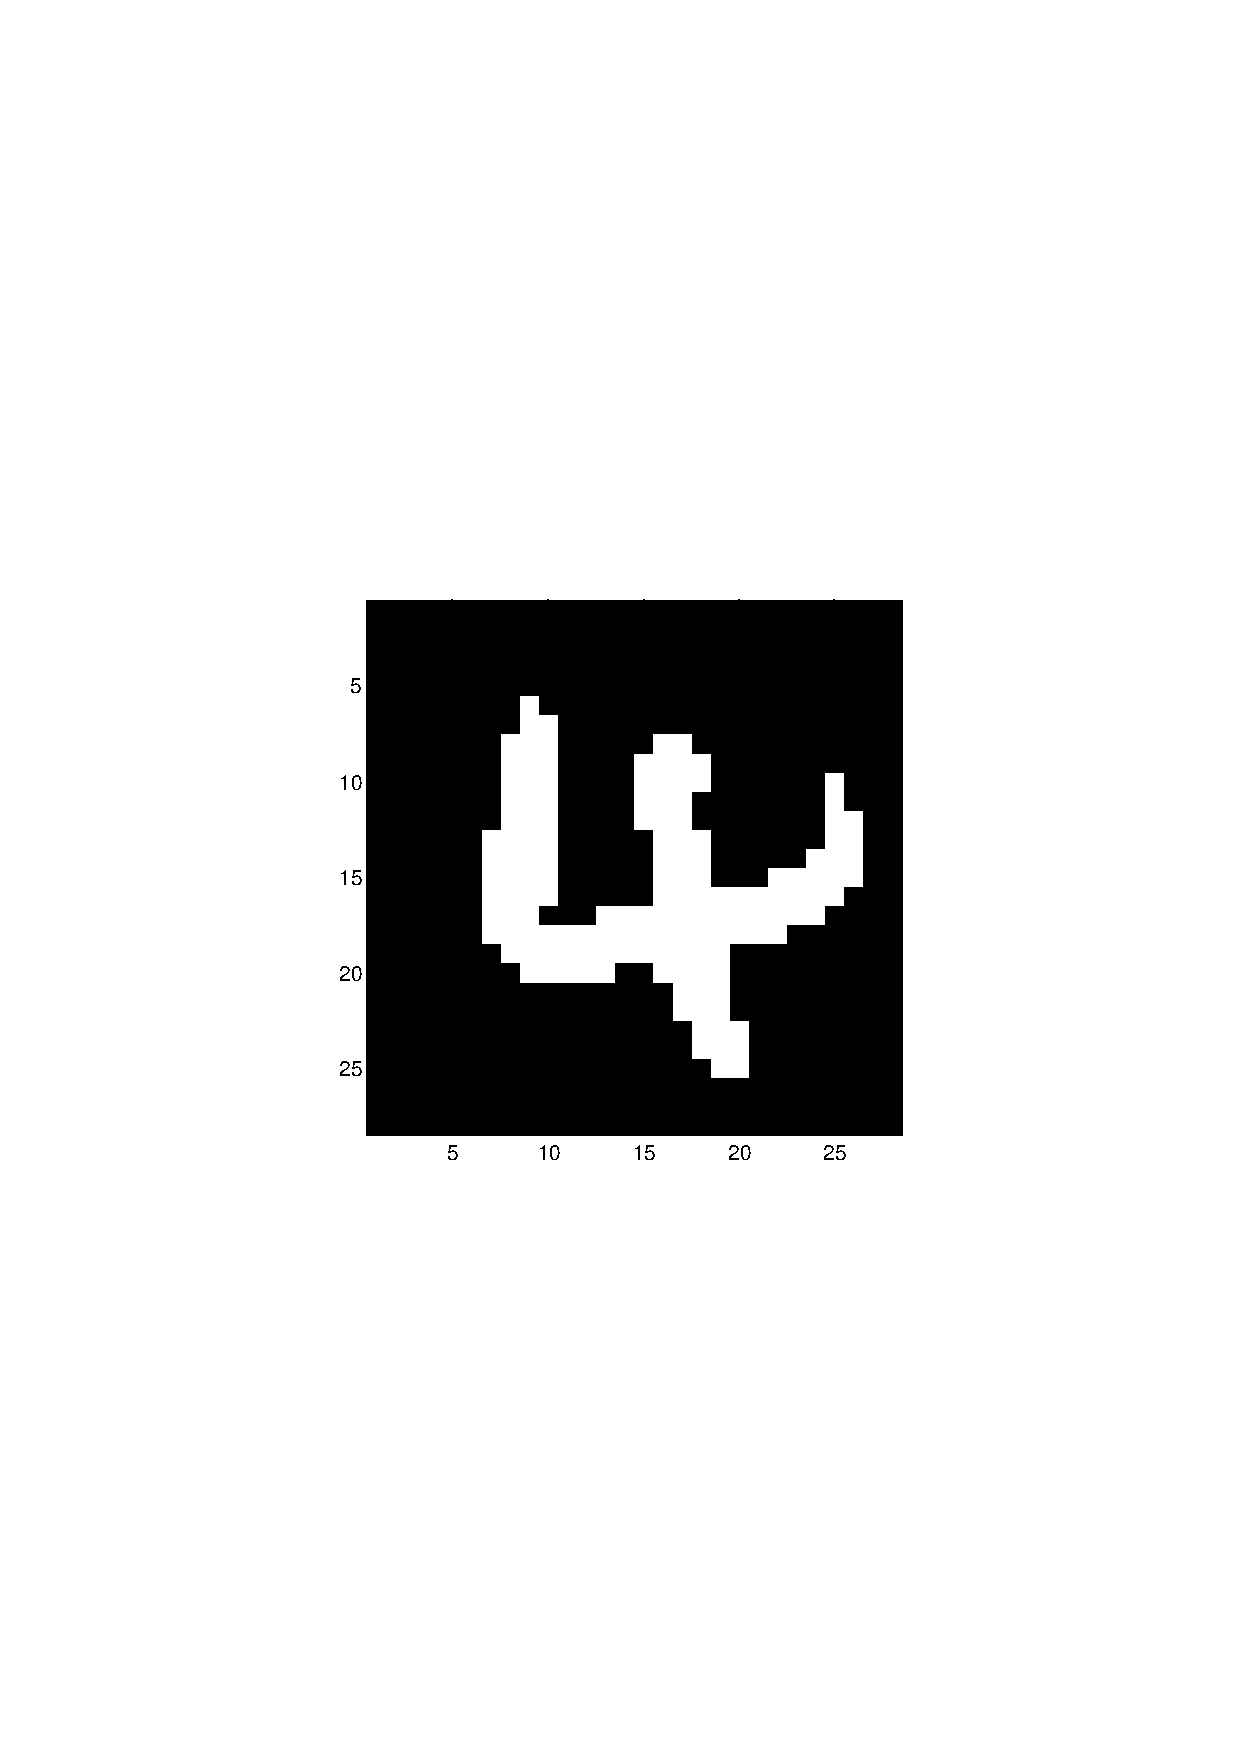
\includegraphics[width=\textwidth]{error_2}
        \end{subfigure}
        ~ %add desired spacing between images, e. g. ~, \quad, \qquad, \hfill etc.
          %(or a blank line to force the subfigure onto a new line)
        \begin{subfigure}[b]{0.3\textwidth}
                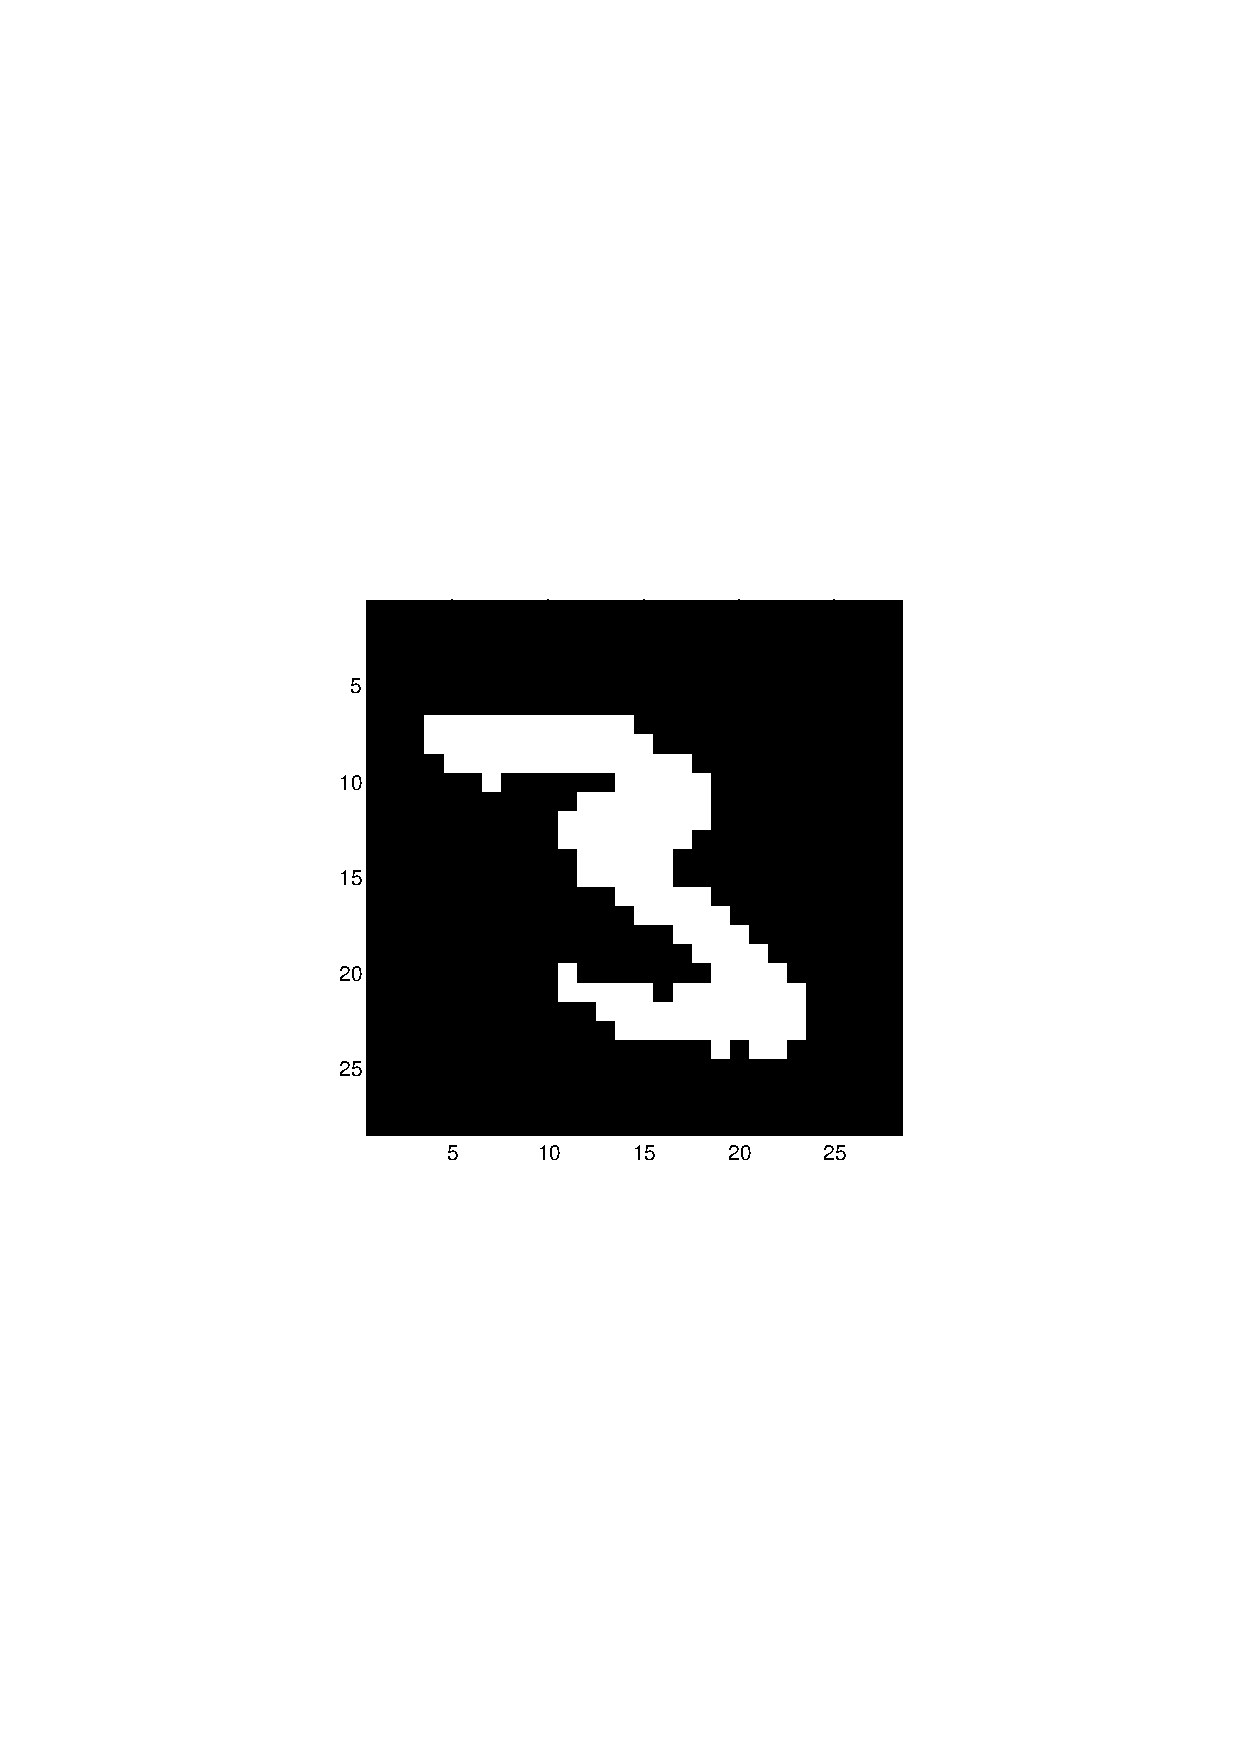
\includegraphics[width=\textwidth]{error_3}
        \end{subfigure}
        \caption{Some examples of the digits in the data set that are misclassified. The first digit is misclassified as a 3, the second digit as a 2 and the third digit as a 2. Looking at the prototypes we can indeed see where the problem lies: in each of these digits there is a big overlap with the wrong digit, either because of the cursive style (digit 3) or because of additional curves (digit 2).}
        \label{error_digits}
\end{figure}

\begin{figure}[H]
	\centering
    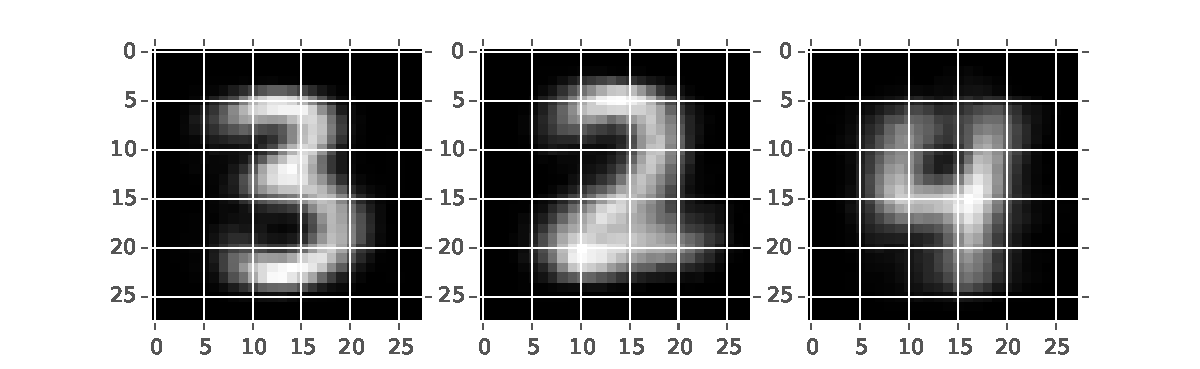
\includegraphics[width=\textwidth]{error_prototypes}
    \caption{The prototypes used in the showing of misclassified digits.}
    \label{error_prototypes}
\end{figure}

\subsubsection{Initializing to true values}
If we initialize the means to the true mean values (as determined by taking the mean of all data points with a certain label), the algorithm converges within 5 iterations. The error is only 4.5\% now.

\begin{minted}[mathescape,
               linenos,
               numbersep=5pt,
               gobble=0,
               frame=lines,
               framesep=2mm,
               fontsize=\footnotesize]{python}
def true_means(data, labels):
	means = np.zeros((3, np.size(data, 1)))
	means[0] = np.mean(np.array([image for index, image in enumerate(data) if labels[index] == 2]), 0)
	means[1] = np.mean(np.array([image for index, image in enumerate(data) if labels[index] == 3]), 0)
	means[2] = np.mean(np.array([image for index, image in enumerate(data) if labels[index] == 4]), 0)

	return means
\end{minted}

\subsubsection{Improving performance}
One way to improve would be to use multiple prototypes for the different variations of a digit. Another way is to use more training data so more variations of the digits are seen. Another way would be to play with the initialization settings and initial mixing coefficients.

\subsection{Customized handwritten digits}
In Photoshop I drew the image as shown in Figure \ref{custom}. Using the following piece of code I classified it using the EM algorithm and the labels:

\begin{minted}[mathescape,
               linenos,
               numbersep=5pt,
               gobble=0,
               frame=lines,
               framesep=2mm,
               fontsize=\footnotesize]{python}
def check_custom_digit(convert, mu, K, pi):
	custom = misc.imread('custom_image.png')
	custom = np.ravel(custom)

	# Initialize gamma array
	gamma = np.zeros((1, K))

	for k in range(0, K):
		gamma[0, k] = pi[k] * bernoulli(custom, mu[k])

	prediction = np.argmax(gamma)
	print "Prediction was: %s" % convert[prediction]
\end{minted}

\begin{figure}[H]
	\centering
    \includegraphics[width=0.2\textwidth]{custom_image.png}
    \caption{The custom digit I drew, representing a 3.}
    \label{custom}
\end{figure}

The digit is consistently misclassified as a 4, even when the prototypes are initialized to their true means. This could be because the middle part of the digit is slightly longer than most 3's.

\end{document}